\documentclass{standalone}
\usepackage[latin1]{inputenc}
\usepackage{tikz}
\usetikzlibrary{automata,positioning, arrows}
\tikzset{->, 
>=stealth, node distance=3cm,every state/.style={thick, fill=gray!10}, % sets the properties for each ’state’ node
initial text=$ $, % sets the text that appears on the start arrow
}
\begin{document}
%    \begin{figure}
    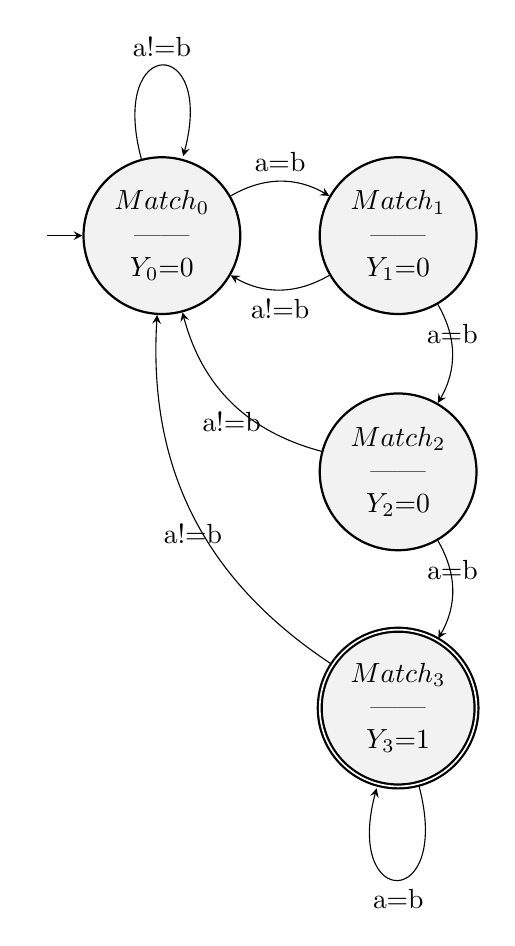
\begin{tikzpicture}
    \node[state,initial,align=center] (Match0) {$Match_0$\\ ------ \\ $Y_0$=0};
    \node[state,right of=Match0,align=center] (Match1) {$Match_1$\\ ------ \\ $Y_1$=0};
    \node[state,below of=Match1,align=center] (Match2) {$Match_2$\\ ------ \\ $Y_2$=0};
    \node[state,accepting,below of=Match2,align=center] (Match3) {$Match_3$\\ ------\\ $Y_3$=1};

    \draw (Match0) edge[loop above] node{a!=b} (Match0)
          (Match0) edge[bend left, above] node{a=b} (Match1)
          (Match1) edge[bend left,above] node{a=b} (Match2)
          (Match2) edge[bend left,above] node{a=b} (Match3)
          (Match3) edge[loop below] node{a=b} (Match3)
          (Match1) edge[bend left,below] node{a!=b} (Match0)
          (Match2) edge[bend left,below] node{a!=b} (Match0)
          (Match3) edge[bend left,below] node{a!=b} (Match0);
    \end{tikzpicture}
%    \caption {FSM diagram of 3 bit sequence detector}
%    \label {Fig.1} 
%   \end{figure}
\end{document}
